\chapter{Designs and Performance Modeling}

Two CNN models - GoogLeNet (inception V1) and Resnet-50 - were implemented on FPGAs in the project. The choices were made based on :  
\begin{itemize}
  \item complexity of CNN models
  \item relevance in the industry
  \item accuracy of the models
  \item availability of pre-trained weights and biases
  \item project timeline
\end{itemize}  
We wanted to implement CNN models complex enough to require scaling over multiple FPGAs. This requirement was a direct consequence of our initial objective of wanting to scale over multiple FPGA devices. Here, the complexity of the model refers the number of hidden layers present in the model. GoogLeNet - with  xyz\todo{Add layer count} layers - and Resnet - with abc \todo{Add layer count} layers- are deep enough to warrant using multiple devices for implementing them.

As the winners of Imagenet Large Scale Visual Recognition Challenge(ILSVR) 2014 and 2015 respectively, GoogLeNet and Reset are quite well known in the industry. With an inference accuracy nearing human capability - GoogLeNet or exceeding human capability -Resnet-152, these models are very popular in the machine learning community. 

Since our objective was to implement an inference engine and not training an inference engine , it was imperative to work with models for which weights and biases were readily available. The popularity of GoogLeNet and Resnet in the machine learning community meant that the weights and biases were available freely in the form of frozen models \todo{Explain frozen models?}.

We stopped at two models as the time required to implement more models was significant and would have forced us to spend less time on other important tasks. And the main objective of our project - implementing CNNs on FPGAs - was met when we successfully implemented GoogLeNet and Resnet. We felt no additional findings would come out of implementing another CNN model on FPGAs.

Implementation of such complex applications on FPGAs calls for "Performance Modeling". Performance Modeling entails the detailed study of how kernels get executed on FPGAs. Performance Modeling allows a design engineer to understand the bottlenecks, performance limiting issues, general performance etc of kernels. Using performance modeling and making an educated assumption about the final design clock frequency, a design engineer can also predict the approximate run-time of a design.
For all the designs which we implemented, we also created models to explain the performance of our designs.    

In the next few sections, we explain in detail how we implemented different FPGA designs of GoogLeNet and Resnet-50 and the accompanying performance models.



\section{GoogLeNet}

The first CNN model we implemented was GoogLeNet. The idea of multiple designs of GoogLeNet was hatched to see the difference in performances when different levels of optimizations are applied at OpenCL level and architectural level. 
We were able implement three major designs for GoogLeNet :
\begin{itemize}
  \item Baseline
  \item DSP Usage Optimized
  \item Hybrid Design
\end{itemize}  

\subsection{GoogLeNet Baseline}

GoogLeNet Baseline was implemented by modifying the OpenCL code generated by TVM for GoogLeNet. We modified the generated code to meet the requirements of our plugin. Some of the major modifications which were performed are :
\begin{itemize}
  \item renaming kernel names
  \item merging ReLUs with Convolutions
  \item rewriting Concatenation layers to support NCHW layout
  \item removing transpose kernels
\end{itemize}  
We had to rename kernels as the naming convention used by TVM and our plugin was not the same. We  had to make sure that we had all the kernels in OpenCL code that the plugin expected to launch.

By merging ReLUs with Convolutions, we optimized away the need to send data from one kernel(Convolutions) to another(ReLUs). This preoptimization step is used in the Deep Learning Community widely as ReLUs are basically light weight operations and do not warrant a separate kernels.

By analysing our plugin, which is an extension to OpenVINO, and TVM, we realized that the layout used by OpenVINO and TVM were quite different. OpenVINO uses NCHW layout scheme whereas TVM uses NHWC layout scheme in Concatenation layer and NCHW layout scheme in all the other layers. To convert from NHWC to NCHW, TVM had generated transpose kernels. We modified all the Concatenation kernels to output NCHW thereby eliminating the need to have transpose layers.  

The modified code was first compiled to run on an FPGA emulator \todo{Insert correct name for emulator}. We verified the functional correctness of the modified code by comparing the values output by our modified code with the values output by TensorFlow implementation of the same model.  

The initial reports generated for this modified OpenCL code indicated that this implementation of GoogLeNet was far too big to fit on a single Stratix 10 board. In order to successfully run this design on FPGAs, there was a need to divide the design into smaller parts. By dividing the design into ten smaller parts, we took advantage of the inherent logical divisions present in GoogLeNet topology. As  described in \ref{GoogLeNet_Topo}, every inception module is followed by a  Concatenation layer. Thus, we divided our design into ten smaller parts.  The first part is a purely feed forward design. The rest of the parts contain at least one inception module each and other layers as shown in Figure \ref{fig:GoogLeNet_division}


\begin{figure}[h!]
  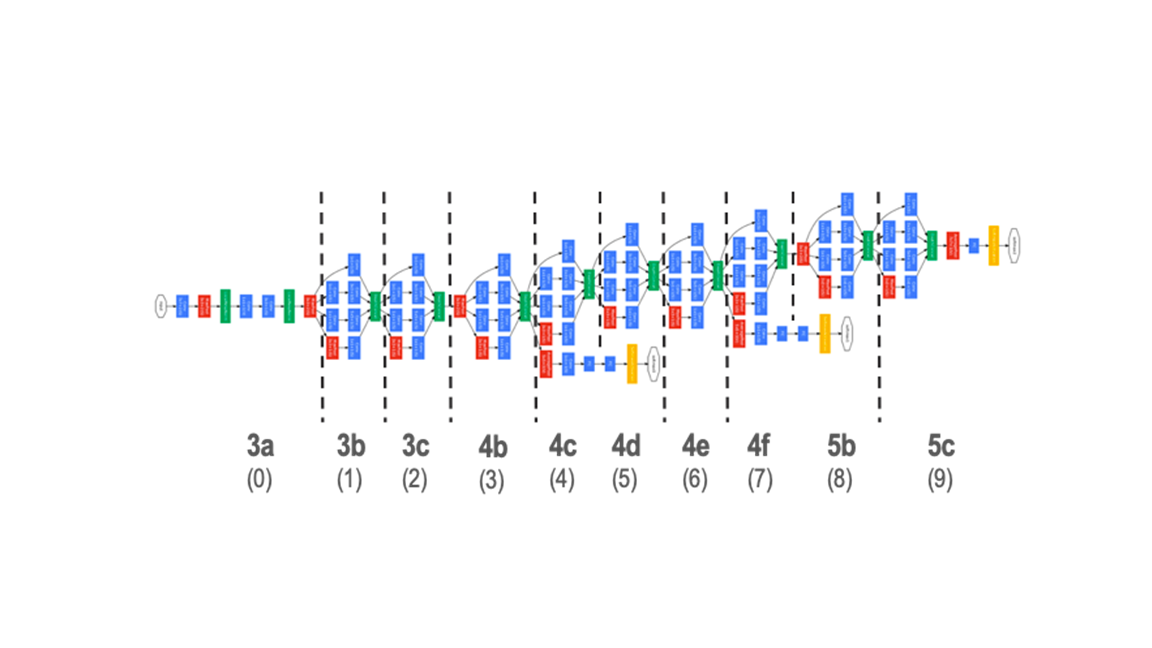
\includegraphics[width=\textwidth,height=\textheight,keepaspectratio]{img/GoogLeNet_division.png}
  \caption{Division of GoogLeNet topology}
  \label{fig:GoogLeNet_division}
\end{figure}
 
The ten resulting OpenCL bitstream files (in aocx format) were named as "inceptionX", where X represents the ordinal value(shown in brackets) of the part the file is made of as shown in Figure \ref{fig:GoogLeNet_division}. For example, the file containing the description of part 3a in Figure \ref{fig:GoogLeNet_division} was named as "inception0.aocx". This naming convention plays a crucial part in deciding the order in which the bitstreams are flashed on multiple devices as discussed further ahead in this section.  

We envisioned scaling over ten devices by using the scheme shown in Figure \ref{fig:GoogLeNet_Scaling}

\begin{figure}[h!]
  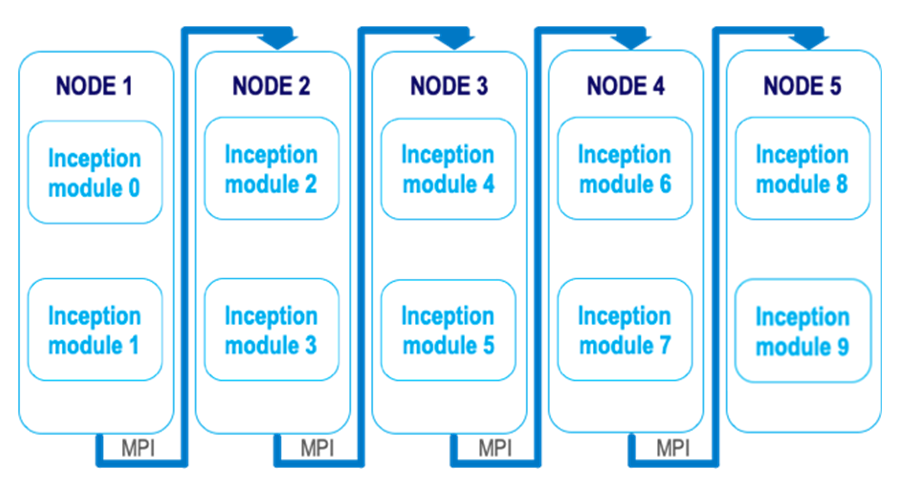
\includegraphics[width=\textwidth,height=\textheight,keepaspectratio]{img/GoogLeNet_Scaling.png}
  \caption{Scaling of GoogLeNet topology over 10 FPGAs}
  \label{fig:GoogLeNet_Scaling}
\end{figure}

Each Noctua FPGA node has two FPGAs. Thus, this scheme requires five nodes to execute ten parts of GoogLeNet. Right off the bat, we had two main challenges - flashing the right bitstreams on to the right devices, and transferring data from one node to another.

The first challenge - flashing the right bitstreams on to the right devices was solved using Message Passing Interface (MPI). This is shown in Listing \ref{code:MPICode_plugin}.  


\begin{code}[!htb]
 \begin{minted}{c++}
 /* Snippet of test plugin - main.cpp */
        #include "mpi.h"
        MPI_Init(NULL,NULL);
        int rank;
        MPI_Comm_rank(MPI_COMM_WORLD,&rank);
        fpga_launcher(network,inputModel,imageNames,cnn_model,rank);
    
\end{minted}
\captionof{listing}{testplugin/main.cpp}
\label{code:MPICode_plugin}
\end{code}

We included the MPI library and initialized it. We retreived the rank of the nodes and then passed the ranks as parameter to the function \texttt{"fpga\_launcher()"}. This function is present in \texttt{"noctua\_plugin /fpga\_plugin.cpp"}. With the ranks as parameters , this function handles the flashing of the bitstreams by calculating the parity of the ranks. These ranks in themselves are enough to identify the nodes(since the ranks are retrieved from the nodes). This is shown in Listing \ref{code:MPICode_fpga_plugin}.

\begin{code}[!htb]
 \begin{minted}{c++}
 /* Snippet of noctua_plugin - fpga_plugin.cpp */
        #include "mpi.h"  
        
        std::string file1 = GoogLeNet_DIR+"inception"+std::to_string(2*rank)+".aocx" 
        std::string file2 = GoogLeNet_DIR+"inception"+std::to_string(2*rank+1)+".aocx"  
        
        std::string file1_xml = GoogLeNet_DIR+"inception"+std::to_string(2*rank)+".xml"
        std::string file2_xml = GoogLeNet_DIR+"inception"+std::to_string(2*rank+1)+".xml"   
        
        char f1_xml[file1_xml.length()];
        strcpy(f1_xml,file1_xml.c_str());  
        
        std::vector<std::string> first_kernels = xml_parser1(f1_xml);

\end{minted}
\captionof{listing}{noctua\_plugin/fpga\_plugin.cpp}
\label{code:MPICode_fpga_plugin}
\end{code}

The naming convention we used for the bitstreams allowed us to pick the appropriate bitstreams by the name and thus, we successfully flashed the bitstreams on to the correct devices. We also read and parsed the XML files which were generated along with the bitstreams. These XML files contain information about the kernels present in a particular bitstream. Using this information, we launched all the valid kernels as needed. 

The second challenge - transferring data from one node to another was also solved using MPI. The devices in a node share the same memory address space and thus , they had access to each other`s global memory.   

The data transfers from one device to another device in the same node were handled using global memory. The data transfers from a device on one node to a deivce on another node was handled using two MPI functions : MPI\_Send() and MPI\_Recv(). We called MPI\_Send() at the last kernel of every node except for the very last one. And the first kernel of every node had a function call for MPI\_Recv(). The visual representation of this scheme is show in Figure \ref{fig:GoogLeNet_Scaling}. Thus, using  MPI\_Send() and MPI\_Recv(), we were able to transfer data from one node to another, allowing us to truly scale over multiple devices.

This implementation of GoogLeNet is completely devoid of optimizations barring a few implementation related optimizations (merging ReLUs with Convolutions etc). Thus, it was named as "Baseline". When we executed this baseline version of GoogLeNet over ten devices, the design took 67.47 seconds to classify one image.  

By any measure, this execution time is extremely slow when it comes to designs running on accelerators. To see why this baseline was slow , we had to first do a performance modelling to explain this run time.

The performance modeling for designs like this involves determining
  Multiply-Accumulate (MAC) operations in design , amount of global memory transfers, run-time, clock frequency and the initiation intervals (IIs) and latency of loops.

The run-time and clock frequency are ascertained from "profile.mon" files.   
The profiling data generated by Intel SDK for OpenCL Applications are stored in files named "profile.mon". These are generated whenever the kernels are executed on FPGAs. During synthesis, it is necessary to enable -profile flag if one wishes to have profiling data generated for their designs (when they are executed on FPGAs). We had enabled this flag for all our designs and thus had access to profiling data for all our kernels.

The first two steps of performance modeling for baseline - determining number of operations and amount of global memory transfers - were done using a script developed by the team. The script was written in Python and made use of ANTLR4 lexer and parser generator tool. OpenCL follows the grammar of C language. Keeping this in mind, we generated a parse tree of all the ten OpenCL source files with the help of ANTLR4 using C.g4 grammar file (Grammar files use the "g4" file extension). We wrote a script to walk the parse tree to determine the number of MAC operations and the amount of global memory transfers present in a file.

The next two steps of performance modeling - determining execution time and clock frequency - were done by opening profile.mon files using the profie.mon viewer provided by Intel SDK for OpenCL. The profiling data records execution time of each and every single kernel which get executed to completion. And the overall frequency at which the kernels in a given OpenCL file run is also recorded in these files.The initiation intervals and latency of different parts of loops is gathered from HTML reports. Taking all this into consideration , the performance modeling of baseline design revealed the details tabulated in Table \ref{tab:GoogLeNetBaselinePerfModel} 
\begin{table}[!htb]                          
 \centering
    \begin{tabular}{|c|c|}
    \multicolumn{2}{c}{\textbf{GoogLeNet Baseline : Performance Model}} \\ \hline

     No.of Operations    &   2.9B \\ \hline
      Global Mem transfers &   20.9 GB            \\ \hline          
      Exe time    &  67470ms    \\ \hline
      Operations/second   &   0.04 GOPS \\ \hline
      Ops/cycle &   0.216             \\ \hline
      Ops/byte       &   0.143     \\ \hline
      Global mem/second & 311 MBps  \\ \hline

    \end{tabular}
    \caption{GoogLeNet Baseline Performance Model}
    \label{tab:GoogLeNetBaselinePerfModel}                            

\end{table}  


The HTML reports revealed that the initiation intervals of most of the loops were much bigger than 1. And some of the loops were not pipelined.There were loop-carried dependencies as well. We also observed from initial reports that the DSP usage of Baseline was quite abysmal. Baseline design was using only about 1\% of the total DSPs available on Stratix 10 board. This is shown in Figure \ref{fig:Report_Baseline}   


\begin{figure}[!htb]
  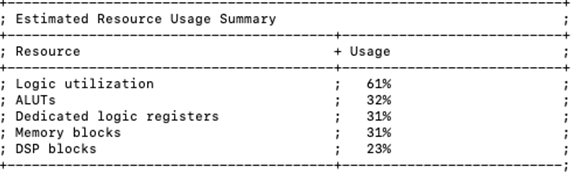
\includegraphics[width=\textwidth,height=\textheight,keepaspectratio]{img/Report_Baseline.png}
  \caption{Initial report of one of the files of Baseline Design}
  \label{fig:Report_Baseline}
\end{figure}

Though the estimated DSP blocks usage is 23\% in Figure \ref{fig:Report_Baseline} , in reality only 1\% of the DSP blocks is used by the design as the overhead required by the board takes up about 22\% of the DSP blocks. The rest remain untouched,unused by our design.

Furthermore, the profiling data for baseline also indicated that the occupancy of  parts of the code where the MAC operations take place were extremely low - in the neighbourhood of 0.1\%. 

Since none of the loops were unrolled, and because of loop carried dependencies (compiler would not unroll automatically), we could estimate that only two operations would take place in one cycle (the inner most loop has two operations - one multiply and one addition). If the loops were unrolled , then the design could have utilized more number of DSP blocks in a single clock cycle thereby executing more number of operations per cycle.   

Additionally, the low utilization of DSP blocks indicates the biggest problem with this design - lack of parallel execution of operations.  

The slowest kernel was at the top of the design - a 3x3 convolution kernel. It took about 18s to get executed. And every other 3x3 convolution kernel took significant amounts of time.

Thus, the reasons for baseline version of GoogLeNet performing so badly were many. To sum it up, the main reasons for slow performance were:
\begin{itemize}
    \item low DSP blocks usage
    \item initiation intervals greater than 1
    \item loop carried dependencies 
    \item global memory transfers
\end{itemize}

To speed this design up, we decided to solve the problem of low DSP usage. This leads us to our next section - GoogLeNet DSP Usage Optimized.

\subsection{GoogLeNet DSP Usage Optimized}



\subsection{GoogLeNet Hybrid Design}

\section{ResNet}
\subsection{ResNet Baseline}
\subsection{ResNet Opt-V1}
\subsection{ResNet Opt-V2}
\subsection{ResNet Opt-V3}
%End of the chapter